\chapter{结论和展望}
\label{chapter:conclusion}
\begin{tikzpicture}[remember picture,overlay]
\node[inner sep=0pt,opacity=0.3] at (current page.center) { % Adjust the opacity here
    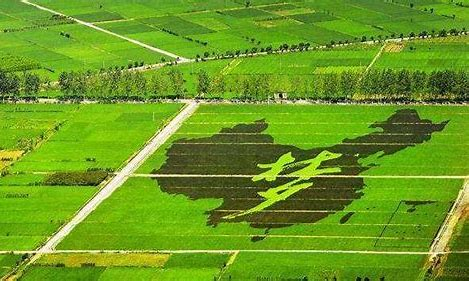
\includegraphics[width=\paperwidth,height=\paperheight]{figures/OIP-C.jpg} % Replace 'background.jpg' with your image file
};
\end{tikzpicture}

在当前的发展阶段,乡村振兴不仅关乎农业、农村和农民的未来,更是国家战略全局的重要组成部分。通过本次数据分析报告,我们得出了一写结论和展望。

必须继续大力稳固粮食安全,这是国家的根本。正如习主席所强调的,“要把中国人的饭碗牢牢端在自己手中”,我们将继续保持粮食生产的稳定性,确保每一粒粮食都能得到妥善利用。

数字农业的发展是提升农业现代化水平的关键。尽管当前数字农业渗透率尚显不足,但我们将加强数字技术在农业中的应用,推动农业生产方式的转变,如《2020年中国农村数字发展报告》所述,通过数字化转型,实现农业的智能化、精准化。

对于偏远地区,推进基础设施建设是实现乡村振兴的前提。我们将加大投资力度,改善交通、水利、电力等基础设施,为乡村发展提供坚实的物质基础。

乡村旅游业的发展是乡村振兴的一大亮点。我们将依托各地的自然风光和文化遗产,打造特色旅游产品,吸引更多游客,带动乡村经济的多元化发展。

优化产业结构,促进私营企业和个体户的发展,是提高农村经济效益的重要途径。我们将制定更多优惠政策,支持乡村产业的创新和升级,增强乡村经济的内生动力。

为促进人口回流,我们将继续完善公共服务,提高农村居民的生活质量,使乡村成为人们向往的美好家园。如习主席所言,“要让农民在乡村振兴中有更多获得感”,我们将努力实现城乡居民的共同富裕。

乡村振兴战略的实施,需要我们在保障粮食安全、推进数字农业、加强基础设施建设、发展乡村旅游业、优化产业结构和促进人口回流等多个方面下功夫。我们将以实事求是的态度,贯彻落实两会精神和三农政策,为实现乡村全面振兴而不懈努力!



